\documentclass[10pt, landscape]{article}
\usepackage[scaled=0.92]{helvet}
\usepackage{calc}
\usepackage{multicol}
\usepackage{ifthen}
\usepackage[a4paper,margin=5mm,landscape]{geometry}
\usepackage{amsmath,amsthm,amsfonts,amssymb}
\usepackage{color,graphicx,overpic}
\usepackage{hyperref}
\usepackage{newtxtext} 
\usepackage{enumitem}
\usepackage{amssymb}
\usepackage[table]{xcolor}
\usepackage{vwcol}
\usepackage{tikz}
\usetikzlibrary{arrows.meta}
\usetikzlibrary{calc}
\usepackage{mathtools}
\usepackage{nicematrix}
\usepackage[T1]{fontenc} %%% <--- NOTE THIS
% for relations
\usepackage{cancel}
\usepackage{ mathrsfs }
\usepackage{listings}
\usepackage{background}
\setlist{nosep}

\usepackage{etoolbox}
\makeatletter
\preto{\@verbatim}{\topsep=0pt \partopsep=0pt }
\makeatother

\backgroundsetup{
scale=1,
color=black,
opacity=0.4,
angle=0,
contents={}
% contents={
\includegraphics[width=\paperwidth,height=\paperheight]{hackerman.png}}
}

\pdfinfo{
  /Title (CS2107.pdf)
  /Creator (TeX)
  /Producer (pdfTeX 1.40.0)
  /Author (Seamus)
  /Subject (Example)
  /Keywords (pdflatex, latex,pdftex,tex)}

\lstset{language=Java,keywordstyle={\bfseries \color{black}}}

% Turn off header and footer
\pagestyle{empty}

\newenvironment{tightcenter}{%
  \setlength\topsep{0pt}
  \setlength\parskip{0pt}
  \begin{center}
}{%
  \end{center}
}

% redefine section commands to use less space
\makeatletter
\renewcommand{\section}{\@startsection{section}{1}{0mm}%
                                {-1ex plus -.5ex minus -.2ex}%
                                {0.5ex plus .2ex}%x
                                {\normalfont\large\bfseries}}
\renewcommand{\section}{\@startsection{section}{2}{0mm}%
                                {-1explus -.5ex minus -.2ex}%
                                {0.5ex plus .2ex}%
                                {\normalfont\normalsize\bfseries}}
\renewcommand{\subsection}{\@startsection{subsection}{3}{0mm}%
                                {-1ex plus -.5ex minus -.2ex}%
                                {1ex plus .2ex}%
                                {\normalfont\small\bfseries}}%
\renewcommand{\subsubsection}{\@startsection{subsubsection}{4}{0mm}%
                                {-1ex plus -.5ex minus -.2ex}%
                                {1ex plus .2ex}%
                                {\normalfont\small\bfseries}}%
\renewcommand{\familydefault}{\sfdefault}
\renewcommand\rmdefault{\sfdefault}
% makes nested numbering (e.g. 1.1.1, 1.1.2, etc)
\renewcommand{\labelenumii}{\theenumii}
\renewcommand{\theenumii}{\theenumi.\arabic{enumii}.}
\renewcommand\labelitemii{•}
%  for logical not operator
\renewcommand{\lnot}{\mathord{\sim}}
\renewcommand{\bf}[1]{\textbf{#1}}
\newcommand{\abs}[1]{\vert #1 \vert}
\newcommand{\Mod}[1]{\ \mathrm{mod}\ #1}

\makeatother
\definecolor{myblue}{cmyk}{1,.72,0,.38}
\everymath\expandafter{\the\everymath \color{myblue}}
% Define BibTeX command
\def\BibTeX{{\rm B\kern-.05em{\sc i\kern-.025em b}\kern-.08em
    T\kern-.1667em\lower.7ex\hbox{E}\kern-.125emX}}
\let\iff\leftrightarrow
\let\Iff\Leftrightarrow
\let\then\rightarrow
\let\Then\Rightarrow

% Don't print section numbers
\setcounter{secnumdepth}{0}

\setlength{\parindent}{0pt}
\setlength{\parskip}{0pt plus 0.5ex}
%% this changes all items (enumerate and itemize)
\setlength{\leftmargini}{0.5cm}
\setlength{\leftmarginii}{0.5cm}
\setlist[itemize,1]{leftmargin=2mm,labelindent=1mm,labelsep=1mm}
\setlist[itemize,2]{leftmargin=4mm,labelindent=1mm,labelsep=1mm}

%My Environments
\newtheorem{example}[section]{Example}
% -----------------------------------------------------------------------

\begin{document}
\raggedright
\footnotesize
\begin{multicols*}{3}

% multicol parameters
% These lengths are set only within the two main columns
\setlength{\columnseprule}{0.25pt}
\setlength{\premulticols}{1pt}
\setlength{\postmulticols}{1pt}
\setlength{\multicolsep}{1pt}
\setlength{\columnsep}{2pt}

\begin{center}
    \fbox{%
        \parbox{0.8\linewidth}{\centering \textcolor{black}{
            {\Large\textbf{CS2107}}
            \\ \normalsize{AY25/26 Sem 1}}
            \\ {\footnotesize \textcolor{myblue}{by ngmh}} 
        }%
    }
\end{center}

\section{Introduction}
\subsection{Security Requirements}
\begin{itemize}
    \item Confidentiality: Prevention of unauthorised disclosure of information
    \item Integrity: Prevention of unauthorised modification of information of processes
    \item Availability: Prevention of unauthorised withholding of information of resources
\end{itemize}

\subsection{Threat Model}
\begin{itemize}
    \item Describe security of a system by the class of attacks it can prevent
    \item A class of attacks is described by the attacker's goals and capabilities
    \item Can be used to compare security of systems
\end{itemize}

\subsection{Trade-Offs}
\begin{itemize}
    \item Ease of Use: Security mechanisms interfere with working patterns users are originally familiar with
    \item Performance: Security mechanisms consume more computing resources
    \item Cost: Security mechanisms are expensive to develop and manage
\end{itemize}

\subsection{Vulnerabilities}
\begin{itemize}
    \item CVE: Common Vulnerabilities and Exposures, public list of entries
    \item Zero Day: Vulnerabilities that are discovered but not published, no reaction time
    \item Adversarial thinking: Thinking like attacker when designing secure systems
\end{itemize}

\subsection{Notions}
\begin{itemize}
    \item Threat: Set of circumstances that has the potential to cause loss or harm
    \item Vulnerability: A weakness in the system
    \item Control: A means to counter threats
    \item A threat is blocked by control of a vulnerability
\end{itemize}

\section{Encryption}
\subsection{Definitions}
\begin{itemize}
    \item Symmetric Key Encryption Scheme: Consists of encryption and decryption algorithm
    \item Correctness: $D_k(E_k(x))=x$
    \item Security (Informally): Eavesdropper cannot derive useful information about key or plaintext even if they can probe
    \item Cryptography: Study of techniques in securing communication in the presence of attackers who have access to it
\end{itemize}

\subsection{Thread Model}
\begin{itemize}
    \item Attacker's Goals:
    \begin{itemize}
        \item Total Break: Attacker wants to find the key
        \item Partial Break: Many definitions, for e.g. attacker wants to decrypt a specific ciphertext
        \item Distinguishability: Attacker can distinguish ciphertexts between one plaintext and another
        \item An attacker who can achieve total break can also achieve partial break and distinguishability
    \end{itemize}
    \item Attacker's capability:
    \begin{itemize}
        \item Ciphertext only: Attacker has a collection of ciphertexts, and may know some properties of it
        \item Known plaintext: Attacker has a collection of plaintexts and corresponding ciphertexts
        \item Chosen plaintext attack (CPA): Attacker has access to encryption oracle, which they can feed any plaintext to to get the corresponding ciphertext
        \item Chosen ciphertext attack (CCA2): Same as CPA but attacker can choose ciphertext to use with decryption oracle to get plaintext
    \end{itemize}
    \item If a cipher can defend against a decryption oracle, then it can defend against all other weaker forms
    \item If a cipher is secure against CCA2, it is also secure against CPA
\end{itemize}

\subsection{Classical Ciphers}
\subsubsection{Substitution Cipher}
\begin{itemize}
    \item The plaintext and ciphertext are strings over a set of symbols
    \item The key is a substitution table which is a bijective function from the set of symbols to itself
    \item The key space is the set of all possible keys with the size being the total number of possible keys
    \item The key size is the number of bits required to represent a key
    \item Encryption: Given plaintext $X=x_1x_2...x_n$ and key $S$, output ciphertext $E_S(X)=S(x_1)S(x_2)...S(x_n)$
    \item Decryption: Given ciphertext $C=c_1c_2...c_n$ and key $S$, output plaintext $D_S(C)=S^{-1}(c_1)S^{-1}(c_2)...S^{-1}(c_n)$
    \item Simple attack is to perform an exhaustive search on the key space
    \item To be secure, exhaustive search must be computationally infeasible
    \item Running time depends on the size of the key space, needing $n!$ loops where $n$ is the size of the alphabet
    \item Known plaintext attack: Attacker has a plaintext and ciphertext, and can use it to reverse engineer some entries in the key
    \item Example would be headers in packets where starting is fixed
    \item Ciphertext only attack: Attacker knows plaintext is an English sentence, so they brute force all keys on the ciphertext, only considering when the result has English words
    \item Frequency analysis: Attacker can guess plaintext by mapping letters to their most frequently occurring counterparts
    \item Substitution cipher is not secure under both types of attacks
\end{itemize}

\subsubsection{Permutation Cipher}
\begin{itemize}
    \item Group plaintext into blocks of $t$ characters then apply a permutation function to each block, where the permutation is a bijective function from $1...t$ to itself
    \item $p=(p_1,p_2,...,p_t)$ which shifts the character $i$ to position $p_i$
    \item Fails miserably under known-plaintext attack
    \item Performing substitution or substitution twice does not increase difficulty of attack, but interlacing them can make it more difficult
\end{itemize}

\subsubsection{One Time Pad}
\begin{itemize}
    \item Encryption: Given $n$ bit plaintext $x_1,...,x_n$ and $n$ bit key $k_1,...,k_n$, $C=(x_1 \oplus k_1),...,(x_n \oplus k_n)$
    \item Decryption: Given $n$ bit ciphertext $c_1,...,c_n$ and $n$ bit key $k_1,...,k_n$, $X=(c_1 \oplus k_1),...,(c_n \oplus k_n)$
    \item Key cannot be reused, but must be same size as plaintext
    \item Correctness is proven by $(x \oplus k) \oplus k = x \oplus (k \oplus k) = (x \oplus 0)=x$
    \item Attacker can derive key with a plaintext and ciphertext pair, but it is useless since keys are only used once
    \item Exhaustive search does not work, and one time pads do not leak any information of plaintext
\end{itemize}

\subsection{Modern Ciphers}
\subsubsection{DES / Exhaustive Search}
\begin{itemize}
    \item Quantify security of encryption scheme by length of key, a scheme with larger keys is more secure wrt exhaustive search
    \item DES uses 56 bit keys, but exhaustive search is now feasible due to improvements in computing power
\end{itemize}

\subsubsection{AES (Advanced Encryption Standard)}
\begin{itemize}
    \item Block length of 128 while key length can be 128, 192, or 256 bits
    \item Currently no known attacks
\end{itemize}

\subsubsection{Block Cipher \& Mode-of-Operations}
\begin{itemize}
    \item DES and AES are block ciphers which are designed for fixed size inputs and outputs
    \item Block cipher is applied to each block in a large plaintext
    \item Mode-of-operation specifies how encryption is extended from a single block to multiple blocks
    \item ECB (Electronic Code Book) mode: Plaintext is divided into blocks before block cipher is applied to each block all with the same key
    \item ECB leaks information, and is deterministic, so additional mechanisms are required to prevent leakage
    \item CBC (Cipher Block Chaining): Intialisation Vector arbitrarily chosen
    \item Encryption: $c_0=IV, c_i=E_k(x_i \oplus c_{i-1}), i>0$ is used to generate ciphertext $y$
    \item Decryption: $P_1 = D_k(C_1) \oplus IV, P_i=D_k(C_i)\oplus C_{i-1}, i>0$
    \item CTR (Counter Mode): Each block $x_i$ uses $IV+i$, at stream cipher
    \item Encryption: $c_i=x_i \oplus E_k(IV+i)$
    \item Decryption: $p_i=c_i \oplus E_k(IV+i)$
    \item GCM (Galois Counter Mode): Authenticated Encryption, produces an extra tag for authentication, secure in presence of decryption oracle
\end{itemize}

% \begin{center}
%     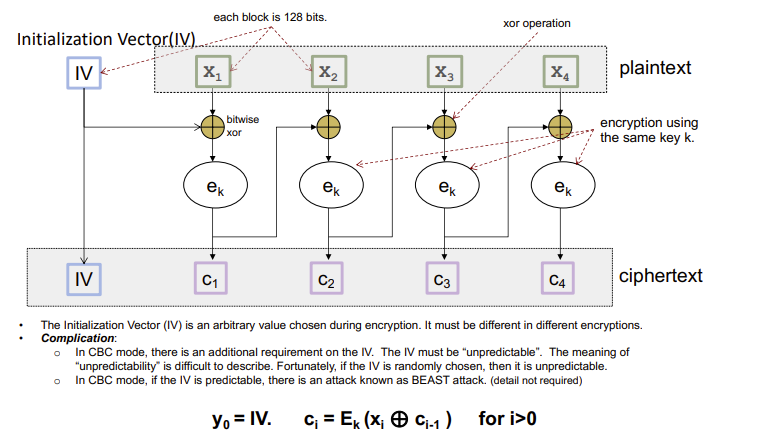
\includegraphics[width=0.5\linewidth]{cbc.png}
%     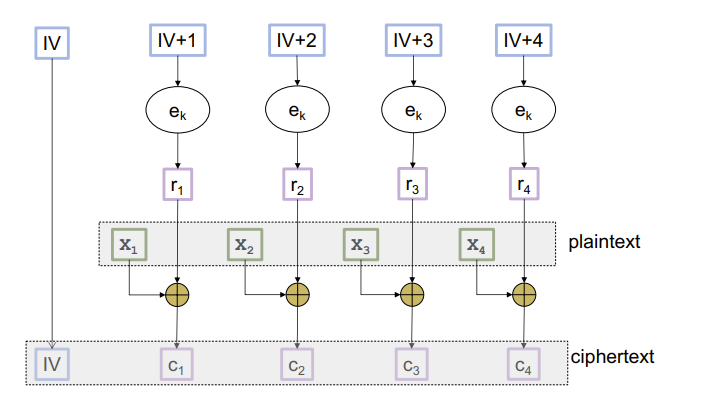
\includegraphics[width=0.5\linewidth]{ctr.png}
% \end{center}

\subsubsection{Stream Cipher and IVs}
\begin{itemize}
    \item Stream cipher has an Intialisation Vector (IV)
    \item Psuerandom sequence is generated from secret key and IV
    \item Final ciphertext contains IV followed by output of OTP encryption
    \item For decryption, IV is extracted from ciphertext, so that same pseudorandom sequence can be generated and used to obtain plaintext
    \item IV should be changed to prevent attacker from eavesdropping and decoding
    \item If IVs are different in two different instances of encryption, the two pseudorandom sequences will also be different, and xoring them will not cancel them out
    \item CBC mode also needs IV for non-determinism
\end{itemize}

\subsection{Attacks}
\subsubsection{Triple DES \& MITM}
\begin{itemize}
    \item DES is not secure wrt computing power, can be improved using multiple encryptions
    \item Meet in the Middle: Attacker brute forces encryption from plaintext with first key and decryption from ciphertext with second key
    \item Tries to find match in the middle
    \item Instead of $2^{2k}$, is now $2^{k+1}$ time
    \item Tradeoff between time and space: Can exhaustively select last $s$ bits of each so that less storage space at $2^{k-s+1}$ but number of operations increases to $2^{s+k+1}$
    \item 3DES: Use triple encryption with 2 keys to make it harder to break, e.g. $E_{k1}(E_{k2}(E_{k1}(x)))$ or $E_{k1}(D_{k2}(E_{k1}(x)))$
\end{itemize}

\subsubsection{Padding Oracle}
\begin{itemize}
    \item An oracle is a query answer system
    \item If length of plaintext is not a multiple of block size, remaining bytes need to be padded, but receiver also needs to know how much padding was used
    \item PKCS\#7 is a padding standard where padding of $x$ bytes is done with $x$ copies of $x$, if block is full an extra block of the block size is added
    \item The padding oracle knows the key and outputs yes if the ciphertext is in the correct padding format
    \item AES CBC is not secure against padding oracle attack
    \begin{itemize}
        \item Attacker knows IV, C, and padding format; padded with $3$ bytes in this case
        \item Attacker calculates iv' from iv by xoring the last 4 bytes where $t$ is set to some value i.e. $0000t777$ to force the padding to flip to $04$
        \item Attacker feeds padding oracle with (iv', c)
        \item If oracle outputs YES, then $x_5 \oplus t$ must be 04, and $x_5$ is $04 \oplus t$
        \item If not, try with another $t$ value
    \end{itemize}
    \item Can be extended to find all plaintexts, only information needed is initial padding length which is easy to determine
    \item Find by flipping from left to right and checking padding
    \item Solution is to deny access to such an oracle, or avoid padding in the first place if possible
    \item CTR mode is also vulnerable to padding oracle attack
\end{itemize}

\subsection{Cryptography Pitfalls}
\begin{itemize}
    \item Wrong choice of IV: e.g. Deriving IV from filename, which can be repeated across different files,should not be same for different ciphertexts
    \item Reusing one time pads
    \item Predictable Secret Generation: Using a fixed seed
    \item Designing your own cipher or modifying an existing scheme; use well-accepted algorithms and libraries
    \item Reliance on Obscurity: Kerckhoff's principle says a system should be secure even if everything about the system other than secret key is known
    \item Security through obscurity is achieving security by hiding system design, but once exposed becomes useless
\end{itemize}

\section{Authentication (Password)}
\begin{itemize}
    \item Authentication: Assuring that communicating entity or origin of information is the one it claims to be, implies integrity
    \item Entity Authentication: For connection-oriented communication, verifying authenticity of entities involved
    \item Data-Origin Authentication: For connectionless communication, verifying origin of a piece of information
    \item Credential: Information bound to owner which is required for authentication, is authentic with owner can convince verifier it has access to it
\end{itemize}

\subsection{Passwords}
\subsubsection{Password System}
\begin{itemize}
    \item Bootstrapping: User and server establish common password, and server keeps a password file recording the users identity and corresponding password
    \item Authentication: Server authenticates an entity by ensuring it gives the correct password
    \item Replay attack: Sniffed information can be replayed to impersonate a user
    \item Password Reset: User can reset password if necessary, but authentication has to be done first
    \item Methods include recovery emails and security questions
\end{itemize}

\subsubsection{Password Attacks}
\begin{itemize}
    \item Attacker can intercept password during bootstrapping or exploit usage of default passwords
    \item Dictionary attack tests all passwords stored in a dictionary and tries all combinations as a form of exhaustive search
    \item Online dictionary attack: Attacker must interact with authentication system while searching (29 bits minimum, 49 bits recommended)
    \item Offline dictionary attack: Attacker obtains some information about password, then carries out search using it without interacting with system through methods such as testing hashes (128 bits minimum)
    \item Social engineering can be carried out to construct a dictionary
    \item Passwords can be stolen through sniffing in various forms such as key loggers or viruses
    \item Phishing attacks are social engineering attacks where the goal is to trick the user to visit a spoofed website and key in their login information
    \item Spear phishing is target to a particular small group of users
    \item Cache usage on platforms like a browser can also leak passwords
    \item If the system administrators account is compromised, password files could also be stolen
    \item Prevention can be done through education and blacklisting phishing sites and using strong passwords
    \item Password Entropy: Measure of strength of password as a measurement of randomness
    \item $-\sum_{i=1}^Np_i log_2p_i$, maximised when probability is uniform
    \item Systems can also have login timeouts or check password strength or require regular password changes, and should also have protected password files using hashing and salting
    \item Passwords generated by human, secret keys generated by machines; key derivation function (KDF) uses password as source for crypto secret key e.g. SHA3
\end{itemize}

\subsection{Biometrics}
\begin{itemize}
    \item Uses physical characteristics of a person for authentication
    \item During enrollment, a template of a user's biometric data is stored, for verification using a matching algorithm
    \item Biometric data acts as password, but has a probability of error
    \item Threshold adjusted for matching algorithm
    \item Can be spoofed, some systems include liveness detection through methods such as temperature sensors
\end{itemize}

\subsection{$n$-factor Authentication}
\begin{itemize}
    \item Uses more than one authentication factor
    \item An example is a password and SMS verification or OTP token
    \item OTP token shares secret with server
    \item Time Based: Based on shared secret and current time interval, a password is generated
    \item Sequence Based: An event triggers change of password
\end{itemize}

\section{Authenticity (Data Origin: MAC \& Signature)}

\subsection{Crypto Primitive: PKC (Public Key Crypto)}
\begin{itemize}
    \item Asymmetric key scheme uses different keys for encryption and decryption
    \item Encryption is done with public key while decryption is done with private key
    \item Only holder of private key can decipher ciphertext
    \item Must be difficult to get private key from public key
    \item Only requires a broadcast channel, does not need a secure channel for sharing of symmetric keys, also uses less keys in total
    \item Authentication is an extremely important part of PKC
    \item Many PKC schemes represent data as integers to which arithmetic operations are applied
\end{itemize}

\subsubsection{RSA}
\begin{itemize}
    \item User chooses large prime $p,q$ and computes $n=pq, \varphi(n)=(p-1)(q-1)$
    \item User randomly chooses an encryption exponent $e$ with $gcd(e, (p-1)(q-1)) = 1$
    \item User finds decryption exponent $d$ where $de\ mod \ (p-1)(q-1)=1$
    \item $(n,e)$ is the public key while $(n,d)$ is the private key
    \item $c=m^e \ mod \ n$ while $m=c^d\ mod \ n$
    \item $D(E(m))=m, m^{ed} \ mod\ n = m$ since $m^{de}\ mod \ n = m\ mod\ n = m$
    \item $e$ and $d$ can have their roles swapped so everyone can decrypt but only owner can encrypt
    \item Common public key is 65537 which is small enough
    \item Difficulty comes from factorising the large value $n$
    \item Post-Quantum Cryptography: PKC that are secure against quantum computers, unlike RSA which will be broken
    \item IVs needed to get different ciphertexts from the same plaintext at different times
    \item Not known whether getting plaintext from ciphertext and public key is as difficult as factorisation
    \item Textbook RSA has to be modified as attacks can use the homomorphic property to extract one bit of information
    \item 128 bit AES and 3072 bit RSA have equivalent key strength, but RSA is significantly slower
    \item PKC is useful for authentication
    \item Typically encrypt AES key with RSA, while using AES to encrypt file instead, send concatenated ciphertext
    \item Other schemes: Discrete log-based PKC such as ElGamal or Paillier Encryption or Lattice-based PKCs
\end{itemize}

\subsection{Data Authenticity (Digest), Unkeyed}
\begin{itemize}
    \item A hash is a function that takes an arbitrary large message as input and outputs a fixed size digest
    \item Collision-Resistant: Difficult to find  different $m_1, m_2$ such that $h(m_1)=h(m_2)$
    \item 2nd Preimage: Given $m_1$, find $m_2$ such that $h(m_1)=h(m_2)$
    \item Preimage: Given $y$, find $m$ such that $h(m)=y$ (one-way)
    \item Popular hash functions are the SHA or MD family
    \item SHA1 and MD5 collisions have been found, use SHA256 or SHA3 instead
    \item Application: Verifying authenticity of file download, attacker tries to find second preimage that is malicious
\end{itemize}

\subsection{Data Origin Authenticity (MAC), Keyed}
\begin{itemize}
    \item A keyed-hash takes an arbitrarily large message and secret key as input and outputs a fixed size message authentication code
    \item Even after seeing multiple valid pairs of messages and MAC, it is still difficult for an attacker to forge an MAC
    \item CBC-MAC: Start with IV $0$ and repeatedly xor with $x_i$ followed by throwing it in $e_k$
    \item Application: When there is no secure channel to deliver digest
    \item Typically MAC is appended to a file and stored together as authentication tag
\end{itemize}

\subsection{Data Origin Authenticity (Signature), Asymmetric Key}
\begin{itemize}
    \item The public key version of MAC is a signature
    \item Owner uses private key to generate signature which public can verify using public key
    \item Easier to manage than MAC
    \item Non-repudiation: Assurance that someone cannot deny previous actions
    \item Popular schemes use RSA for signing and verifying
    \item Signature schemes consist of unkeyed hash followed by signing and verifying algorithm
    \item With RSA, $s=RSA_E(key^-, H(x))$, $(X,s)$ can be verified by checking $H(X)=RSA_D(key^+, s)$
    \item Some signature schemes do not use encryption in their scheme
\end{itemize}

\subsection{Attacks and Pitfalls}
\begin{itemize}
    \item Birthday Attacks: Repeatedly generate messages until probability of finding collision is high
    \item Suppose we have $M=1.17\cdot2^{64}$ messages and each has a value from $T=2^{128}$, the probability of collision is $1-e^{(-\frac{M^2}{2T})}$, this gives $P>0.5$, basically half the bits
    \item For a set of $k$ distinct elments of $n$ bits, select $m$ of them and put them in another set. The probability of non-empty intersection is $>1-2.7^{-km2^{-n}}$
    \item Using encryption for authentication: Encryption provides confidentiality, but not integrity or authenticity
\end{itemize}

% stopped here

% \section{PKI (Public Key Infrastructure) \& Channel Security}
% \subsection{Public Key Distribution}
% \begin{itemize}
%     \item Both public keys and symmetric keys require a secure channel to distribute keys, but it is easier to securely broadcast public keys that do not require both entities to interact
%     \item Public Announcement: Owner broadcasts public key, but not standardised, and there is no systematic way to search and verify them
%     \item Publically Available Directory: Directory server which supports lookup, but server cannot verify that information is authentic
% \end{itemize}

% \subsection{Public Key Infrastructure}
% \begin{itemize}
%     \item Standardised system to distribute public keys
%     \item Centered around Certificate and Chain of trust of Certificate Authority (CA)
% \end{itemize}

% \subsubsection{Certificate Authority}
% \begin{itemize}
%     \item A CA issues certificates
%     \item Trusted authority that manages directory of public keys
%     \item Has its own public and private key pair, which still needs a secure channel to distribute
%     \item Most OSes and browsers have a few pre-loaded CA's public keys (root CAs)
%     \item Without certificate: User has to take other user's public key and compare it without result of query with CA
%     \item With certificate: User can check certificate and verify signature in certificate belongs to CA, does not need to query CA
%     \item A certificate contains at least a name, public key of owner, time window of validity, and signature of CA
%     \item Standardisation Bodies specify formats for certificates
%     \item A self-signed certificate is signed by its owner and is to be verified using public key listed in certificate
%     \item Convenient in manual installation of public key
% \end{itemize}

% \subsubsection{Trust Relationship}
% \begin{itemize}
%     \item CA also has to verify that information is correct before issuing certificate, could be costly
%     \item If user does not have public key of CA of a certificate, needs to obtain it from other CAs
% \end{itemize}

% \subsubsection{Revocation}
% \begin{itemize}
%     \item Certificates can be revoked for various reasons such as private key being compromised, CA being compromised, or entity closing / leaving
%     \item Verifier needs to check validity of certificate even if it is not expired
%     \item Certificate Revocation List: CA periodically signs and publishes list of revocations
%     \item Online Certificate Status Protocol: OCSP responder validates a certificate in question
%     \item Either way, some online check has to be done, maybe periodically
% \end{itemize}

% \subsection{Limitations of PKI}
% \begin{itemize}
%     \item Implementation bugs can lead to vulnerabilities, such as browsers truncating after null characters
%     \item Malicious CAs can forge certificates
%     \item Social engineering exploits confusing naming to trick verifiers into using a wrong name such as typosquatting or sub-domains
% \end{itemize}

% \subsection{Authentication}
% \begin{itemize}
%     \item Attack Model: Sniff-then-impersonate
%     \item Weak Authentication: Passwords can be replayed for impersonation
%     \item Challenge-Response: Verifier issues a random challenge which entity has to respond to correctly, ensuring freshness using cryptographic nonce
%     \item Unilateral Authentication using PKC: Public key version using signatures using signature of random message and certificate
%     \item Authenticated key exchange: First phase produces a session key, which is then used for protecting communication with encryption and MAC
% \end{itemize}

% \subsection{Key-Exchange}
% \begin{itemize}
%     \item PKC-Based:
%     \begin{itemize}
%         \item Alice generate private and public key pair
%         \item Alice sends public key to Bob
%         \item Bob chooses a session key, encrypts it, and sends it to Alice
%         \item Alice decrypts it to obtain the session key
%         \item Attacker cannot get session key
%     \end{itemize}
%     \item Diffie-Hellman Key-Exchange:
%     \begin{itemize}
%         \item Agree on generator $g$ and large prime $p$
%         \item Alice randomly chooses $a$ and transmits $x=g^a\ mod \ p$
%         \item Bob randomly chooses $b$ and transmits $y=g^b\ mod\ p$
%         \item Alice computes $k=y^a\ mod \ p$
%         \item Bob computes $k=x^b\ mod\ p$
%         \item Assumption: It is computationally infeasible to find $k=g^{ab}\ mod\ p$ given $g,p,x,y$
%     \end{itemize}
% \end{itemize}

% \subsection{Authenticated Key-Exchange}
% \begin{itemize}
%     \item Basic key exchange can be attacked by an impersonator in the middle
%     \item Can be done using key-exchange by signing all communication with private keys
%     \item Authenticated key-exchange using DH: Station to Station Protocol
%     \item To authenticate Bob, Bob signs $y$ to obtain a signature which Alice will verify after transmission using Bob's keys
%     \item Can also be done with symmetric keys and passwords
% \end{itemize}

% \subsection{Secure Communication Channel}
% \begin{itemize}
%     \item Public channel is not secure with presence of attackers
%     \item TLS/SSL: Use long-term keys to carry out authenticated key-exchange (handshake) so that they both have a session key
%     \item Subsequent communication is protected by this session key
%     \item Alice obtains Bob's public key from Bob's certificate
%     \item Alice and Bob carry out unilateral authenticated key exchange with Bob's keys, obtaining session keys $t$ for MAC and $k$ for symmetric key encryption such as AES
%     \item Subsequent interactions use $t,k,$ and a sequence number with information sent being $E_k(i | m)|MAC_t(E_k(i |m))$ (encrypt-then-MAC)
%     \item SSL is the predecessor of TLS, HTTPS is built on top of TLS
% \end{itemize}

% \section{Network Security}
% \subsection{Computer Networking}
% \begin{itemize}
%     \item Establishes communication between entities
%     \item Uses packet switching where messages route via switches and routers, broken up into packets
%     \item Uses routing to decide how to route messages using intermediate nodes
%     \item Each node has different names in different layers; domain name, port number, ip address, mac address
%     \item Protocol in a layer might transform a message into multiple payloads using a lower layer to transfer it before reconstruction
%     \item Man-In-The-Middle sits between two communicating parties and can sniff, spoof, modify, or drop data
%     \item L3: MITM can see datagram and transport header, has access to internal data
%     \item Between L2 and L3: Can see and modify output of L3 but does not have access to internal data
%     \item Leakage of routing information could reveal connectivity information which does not provide anonymity and privacy
%     \item Processes are identified by ip address and port
%     \item UDP: Sends datagrams in packets to destination address, but with no delivery guarantee
%     \item TCP: Reliable, handshake established to make sure connection is successful
% \end{itemize}

% \subsection{Name Resolution and Attacks}
% \begin{itemize}
%     \item DNS (Domain Name System): Resolves domain names into IP addresses
%     \item ARP (Address Resolution Protocol): Resolves IP address to MAC address
%     \item DNS Spoofing: Attacker replies DNS query with another malicious IP address
%     \item Switches connects ports based on MAC addresses
%     \item ARP Poisoning: Attacker inserts false entries into ARP tables so that packets are mistakenly sent to it
% \end{itemize}

% \subsection{Denial of Service Attack}
% \begin{itemize}
%     \item Attack on availability, preventing authorised access to resources or delaying time critical operations
%     \item Send large number of http requests to a server, or large number of DNS requests to DNS server
%     \item When carried out by a large number of attackers, known as Distributed DOS
%     \item Reflection: DOS where attackers send requests to intermediate nodes, in turn sending overwhelming traffic to victim
%     \item Amplification factor: Size of traffic victim received over size of traffic send by attacker
%     \item ICMP/Smurf flood: Attacker sends ICMP ping with source IP of victim, causing all entities who receive broadcast to reply
%     \item DNS reflection using multiple DNS resolvers is also possible
%     \item Bot: Compromised Machine, Botnet: Large collection of connected bots, which has a command and control mechanism and can be used for attacks such as DDOS
% \end{itemize}

% \subsection{Tools}
% \begin{itemize}
%     \item Wireshark: Used to analyse packets, capturing interactions between OS and network card
%     \item nmap: Used for portscanning
% \end{itemize}

% \subsection{Protection using Cryptography}
% \begin{itemize}
%     \item Different protocols protect different layers
%     \item SSL/TLS sits on the transport layer and protects data with encryption and MAC
%     \item Wifi Protected Access II (WPA2): Provide protection in layer 2 (link) and layer 1 (physical), but not all information in layer 2 is protected
%     \item IPSec: Mechanism whcih aims to protect layer 3 (IP)
%     \item Typical implementations use TLS/SSL + WPA2 since IPSec is expensive and difficult to deploy
%     \item Virtual Private Network: Virtually become a node in a network by establishing a tunnel between transport layer of client and VPN server
% \end{itemize}

% \subsection{Firewalls}
% \begin{itemize}
%     \item Divide network into segments and deny unnecessary access
%     \item Principle of Least Privilege: Every module must be able to access only information and resources needed for legitimate purposes
%     \item Compartmentalisation: Confining information within compartments
%     \item A firewall controls what traffic is allowed to enter or leave the network (ingress and egress filtering)
%     \item DMZ: Demilitarised zone; a sub-network exposing organisations external service to the internet
%     \item Firewalls perform packet filtering which inspects every packet
%     \item Deep Packet Inspection: Inspecting payload as well, not just headers
%     \item Example rules are checking source IP, and whitelists or blacklists
%     \item Rules are defined by matching conditions and actions
%     \item Types: Packet filters, Stateful inspection, Proxy
%     \item Intrusion Detection System: Set of sensors which gather data, to be analysed for intrusion
%     \item Attack signature detection: Attack has specific well defined signature
%     \item Anomaly detection: Attempt to detect abnormal patterns
%     \item Behaviour based: A type of anomaly detection focusing on human behaviour
% \end{itemize}

% \subsection{Management}
% \begin{itemize}
%     \item Needed to monitor and adjust network characteristics
%     \item SOC: Security Operations Center, monitors IT systems and deals with security issues
% \end{itemize}

% \section{Access Control}
% \subsection{Access Control Model}
% \begin{itemize}
%     \item Restrict operations on objects by subjects
%     \item Security Parameter: Access control sets it up so that malicious activities outside it will not affect resources within it
%     \item Design uses Principle of Least Privilege, Compartmentalisation, Defense in depth, and Segregation of duty
%     \item Defense in Depth: Use multiple layers so that if one fails perimeter is still not compromiseds
%     \item Segregation of Duty: Assign different components to different people so that there will not be a single point of failure
%     \item Principal / Subject wants to access an object with some operation
%     \item Reference monitor either grants or denies the access
%     \item Principals are human users while subjects are entities acting on behalf of them
%     \item Some accesses are observation, alteration, or actions
%     \item Every object has an owner, with access rights either being decided by owner (discretionary access control) or system-wide policies (mandatory access control)
% \end{itemize}

% \subsection{Access Control Matrix}
% \begin{itemize}
%     \item How to specify access rights of a particular principal to a particular object
%     \item Use access control matrix to show; one axis principals and the other objects
%     \item ACL: Access control list rather than matrix, for each file
%     \item Capabilities: Subject has a list of capabilities, each for a specific object
%     \item Capability: Unforgeable token that gives possessor certain rights to an object
% \end{itemize}

% \subsection{Intermediate Control}
% \begin{itemize}
%     \item Specifying every single entry in the access control matrix is tedious
%     \item Grouping subjects and objects and defining access rights on the group simplifies it and is known as intermediate control
%     \item Unix has permissions for owner, group, and world
%     \item Grouping can be determined by role of subject, associated with a collection of procedures
%     \item Privilege is often called protection rings, which are the same but with different names
%     \item A subject with a lower number has higher privilege
%     \item Bell-LaPadula Model for data confidentiality: No read up or write down, prevents lower level from getting information from higher level, and malicious insider from passing information to lower levels
%     \item Biba Model for process integrity: No write up or read down, prevents malicious subjects from poisoning upper level data, and prevents subject from reading data poisoned by lower level subjects
% \end{itemize}

% \subsection{Unix File System}
% \begin{itemize}
%     \item Objects include files, directories, memory devices, and I/O devices
%     \item File System Permission: Grouped into 3 triples; read, write, execute, for owner, group, world
%     \item File Permission, Links Count, Owner ID, Group ID, File Size, Data and time of last modification, Filename
%     \item Principals are user identities and group identities, with their information stored in password file which is world readable
%     \item Subjects are processes, each with a PID
%     \item Unix has 2 protection rings: superuser which has no security checks, and user
%     \item On access, check if user is owner and owner permission bits, then if user group owns file, check group permission bits, if not check the world permission bits
% \end{itemize}

% \subsection{Controlled Invocation \& Privilege Escalation}
% \begin{itemize}
%     \item Controlled Invocation: Allow user to access a file temporarily
%     \item System provides a predefined set of applications with access to a file
%     \item Application is granted elevated privilege so it can freely access a file and any user can invoke it
%     \item Developer has responsibility to ensure that application only performs intended operation
%     \item Can view predefined application as bridge between user and sensitive data
%     \item Privilege Escalation Attack: Attacker tricks bridge to perform illegal operations
% \end{itemize}

% \subsection{Controlled Invocation in UNIX}
% \begin{itemize}
%     \item A process is a subject with a PID, which can be created by executing a file or forking an existing process
%     \item A process is associated with a Real UID and Effective UID
%     \item Real UID is inherited from user who invokes the process
%     \item If Set User ID is disabled, process effective UID is same as real UID
%     \item If enabled, process effective UID is inherited from UID of file owner
%     \item When process wants to access a file, effective UID of process is treated as subject and checked against file permission to determine whether it has access
%     \item SUID must be enabled in file permissions
%     \item Process is temporarily elevated to superuser so it can access the sensitive data
% \end{itemize}

% \section{Call Stack}
% \begin{itemize}
%     \item Von Neumann Computer Architecture, code is treated as data and both are stored in the same memory
%     \item Program counter is a register that stores address of next instruction
%     \item After an instruction is executed, processor fetches another instruction from memory, and program counter is incremented
%     \item Direct branch: Program counter replaced by constant value
%     \item Indirect branch: Program counter replace by value fetched from memory
% \end{itemize}

% \subsection{Control Flow Integrity}
% \begin{itemize}
%     \item Attacker can compromise execution by modifying code in memory or modifying the address for indirect branching
%     \item First attack is overwriting executing code with malicious code
%     \item Second is overwriting a piece of control flow information for either a direct or indirect jump
%     \item Modifying a code address used by an indirect jump is known as stack smashing
% \end{itemize}

% \subsection{Call Stack}
% \begin{itemize}
%     \item Call stack stores information of function calls in stack frames
%     \item Stack pointer stores location of the top of the stack
%     \item Call stack keeps track of parameters passed, control flow information such as return address, local variables of functions, pointer to previous stack frame
%     \item Stack Smash: Attacker can modify stack with a buffer overflow
% \end{itemize}

% \section{Secure Programming}

% \subsection{printf Vulnerabilities}
% \begin{itemize}
%     \item Uses a format string and parameters
%     \item When format specifier is found in format string, program fetches value of parameter and displays it, even if a second parameter is not given to printf
%     \item By calling printf with a user specified string, an attacker can inject format specifiers to extract information or cause a crash or modify memory content, especially if the program is run with elevated privileges
% \end{itemize}

% \subsection{Data Representation}
% \begin{itemize}
%     \item Inconsistencies in data representation can cause vulnerabilities
%     \item C strings are represented with null characters marking the end
%     \item A system using both null and non-null definitions might get confused
%     \item Consider a browser which verifies certificates with non-null termination and displays name with null termination
%     \item Attacker can spoof a certificate which has name displayed correctly because an extra null character is inserted
%     \item Do not trust user input, user canonical representations
% \end{itemize}

% \subsection{Buffer Overflow}
% \begin{itemize}
%     \item C and C++ do not check array bounds at runtime
%     \item A buffer overflow is when data is written beyond a buffer's boundary
%     \item strcpy is an unsafe function because it does not do bounds checking
%     \item Stack smashing is a buffer overflow targeting the call stack
% \end{itemize}

% \subsection{Integer Overflow}
% \begin{itemize}
%     \item Incrementing a number beyond its maximum value usually loops over to its minimum value
%     \item Some invariants might not hold and can lead to vulnerabilities
% \end{itemize}

% \subsection{Code Injection}
% \begin{itemize}
%     \item Scripting languages automate execution that could be executed line by line by a human, and are typically interpreted rather than compiled
%     \item Many scripting languages allow scripts to be stored data
%     \item The most well known is an SQL injection
%     \item Malicious user can write SQL inside an input field which causes it to be executed
% \end{itemize}

% \subsection{Undocumented Access Point}
% \begin{itemize}
%     \item Developers might leave backdoors for debugging purposes
%     \item These might accidentally be left in the production build
%     \item Also known as easter eggs
% \end{itemize}

% \subsection{Race Condition}
% \begin{itemize}
%     \item Occurs when multiple processes access a piece of shared data in such a way that outcome depends on order of access
%     \item Time of check time of use race condition is when another process is completed between these two time points
%     \item Example: First program does verification before access, and second program modifies resource being accessed between these two time points
% \end{itemize}

% \subsection{Defense and Preventive Measures}
% \begin{itemize}
%     \item Input validation, Filtering, Parameterised Queries: Perform input validation whenever an input is obtained from user with a whitelist or blacklist
%     \item Use safe functions rather than unsafe versions which have vulnerabilities
%     \item Bound Checks: Before accessing a location, ensure that it is within bounds
%     \item Type Safety: Ensure that arguments to an operation are always of the correct type
%     \item Canaries: Secrets inserted at selected memory locations during runtime to ensure that values are not being modified
%     \item Memory Randomisation: Address space layout randomisation makes it harder for attacker to know location of data and code for modification
%     \item Code Inspection: Manual or automated checking which checks whether input to critical functions could be affected by user inputs
%     \item Testing: White-box, black-box, grey-box testing
%     \item Fuzzing: Send malformed inputs to discover vulnerabilities
%     \item Principle of Least Privilege
%     \item Patching: Quickly applying patches to fix vulnerabilities when they are found
% \end{itemize}

% \section{Web Security}
% \begin{itemize}
%     \item Complicated due to browsers wide range of support and dealing with sensitive information
%     \item Threat Model 1: Attackers are other end systems
%     \item Thread Model 2: Attackers are MITM
%     \item Vulnerability in Secure Communication Channel: Assumption that system is designed and implemented correctly
%     \item Misleading user with domain name: No clear distinction between hostname and path, can be spoofed using characters that look like /
%     \item Address bar spoofing: In a poorly designed browser, attackers could spoof address bars
%     \item Cookies can have a same origin policy which means it is only sent back to the server that set it
%     \item Same origin policies have confusing definitions which might not be the same between browsers
%     \item Cross Site Scripting: Injecting code in a url that gets run for example through a content render, allowing attacker to deface webpage or steal cookies and make requests
%     \item Can be reflection or stored XSS, for example in a forum page
%     \item Cross Site Request Forgery: Exploits server's trust of client by sending a modified request which benefits attacker, can be prevented with authentication
% \end{itemize}

% \subsection{Other Attacks and Terms}
% \begin{itemize}
%     \item Drive by Download: Download happening without user consent
%     \item Web Bug: Tiny object embedded in webpage to track user behaviour
%     \item Clickjacking: User tricked into clicking something different from what they actually are
%     \item CAPTCHA: Challenge response test to verify a user is human
%     \item Click Fraud: Malicious actos click on ads to generate fake revenue or drain a competitors budget
% \end{itemize}

% \subsubsection{Common Implementation Mistakes}
% \begin{itemize}
%     \item Authentication and filtering on client side
%     \item Security credentials embedded in public web pages
%     \item Server secrets stored in cookies
%     \item Configuration errors
%     \item URL as secrets without adequate protection
% \end{itemize}

\end{multicols*}

\end{document}